% Options for packages loaded elsewhere
\PassOptionsToPackage{unicode}{hyperref}
\PassOptionsToPackage{hyphens}{url}
%
\documentclass[
]{book}
\usepackage{lmodern}
\usepackage{amssymb,amsmath}
\usepackage{ifxetex,ifluatex}
\ifnum 0\ifxetex 1\fi\ifluatex 1\fi=0 % if pdftex
  \usepackage[T1]{fontenc}
  \usepackage[utf8]{inputenc}
  \usepackage{textcomp} % provide euro and other symbols
\else % if luatex or xetex
  \usepackage{unicode-math}
  \defaultfontfeatures{Scale=MatchLowercase}
  \defaultfontfeatures[\rmfamily]{Ligatures=TeX,Scale=1}
\fi
% Use upquote if available, for straight quotes in verbatim environments
\IfFileExists{upquote.sty}{\usepackage{upquote}}{}
\IfFileExists{microtype.sty}{% use microtype if available
  \usepackage[]{microtype}
  \UseMicrotypeSet[protrusion]{basicmath} % disable protrusion for tt fonts
}{}
\makeatletter
\@ifundefined{KOMAClassName}{% if non-KOMA class
  \IfFileExists{parskip.sty}{%
    \usepackage{parskip}
  }{% else
    \setlength{\parindent}{0pt}
    \setlength{\parskip}{6pt plus 2pt minus 1pt}}
}{% if KOMA class
  \KOMAoptions{parskip=half}}
\makeatother
\usepackage{xcolor}
\IfFileExists{xurl.sty}{\usepackage{xurl}}{} % add URL line breaks if available
\IfFileExists{bookmark.sty}{\usepackage{bookmark}}{\usepackage{hyperref}}
\hypersetup{
  pdftitle={Mulling Over McElreath's Statistical Rethinking},
  pdfauthor={Dan Burrell},
  hidelinks,
  pdfcreator={LaTeX via pandoc}}
\urlstyle{same} % disable monospaced font for URLs
\usepackage{color}
\usepackage{fancyvrb}
\newcommand{\VerbBar}{|}
\newcommand{\VERB}{\Verb[commandchars=\\\{\}]}
\DefineVerbatimEnvironment{Highlighting}{Verbatim}{commandchars=\\\{\}}
% Add ',fontsize=\small' for more characters per line
\usepackage{framed}
\definecolor{shadecolor}{RGB}{248,248,248}
\newenvironment{Shaded}{\begin{snugshade}}{\end{snugshade}}
\newcommand{\AlertTok}[1]{\textcolor[rgb]{0.94,0.16,0.16}{#1}}
\newcommand{\AnnotationTok}[1]{\textcolor[rgb]{0.56,0.35,0.01}{\textbf{\textit{#1}}}}
\newcommand{\AttributeTok}[1]{\textcolor[rgb]{0.77,0.63,0.00}{#1}}
\newcommand{\BaseNTok}[1]{\textcolor[rgb]{0.00,0.00,0.81}{#1}}
\newcommand{\BuiltInTok}[1]{#1}
\newcommand{\CharTok}[1]{\textcolor[rgb]{0.31,0.60,0.02}{#1}}
\newcommand{\CommentTok}[1]{\textcolor[rgb]{0.56,0.35,0.01}{\textit{#1}}}
\newcommand{\CommentVarTok}[1]{\textcolor[rgb]{0.56,0.35,0.01}{\textbf{\textit{#1}}}}
\newcommand{\ConstantTok}[1]{\textcolor[rgb]{0.00,0.00,0.00}{#1}}
\newcommand{\ControlFlowTok}[1]{\textcolor[rgb]{0.13,0.29,0.53}{\textbf{#1}}}
\newcommand{\DataTypeTok}[1]{\textcolor[rgb]{0.13,0.29,0.53}{#1}}
\newcommand{\DecValTok}[1]{\textcolor[rgb]{0.00,0.00,0.81}{#1}}
\newcommand{\DocumentationTok}[1]{\textcolor[rgb]{0.56,0.35,0.01}{\textbf{\textit{#1}}}}
\newcommand{\ErrorTok}[1]{\textcolor[rgb]{0.64,0.00,0.00}{\textbf{#1}}}
\newcommand{\ExtensionTok}[1]{#1}
\newcommand{\FloatTok}[1]{\textcolor[rgb]{0.00,0.00,0.81}{#1}}
\newcommand{\FunctionTok}[1]{\textcolor[rgb]{0.00,0.00,0.00}{#1}}
\newcommand{\ImportTok}[1]{#1}
\newcommand{\InformationTok}[1]{\textcolor[rgb]{0.56,0.35,0.01}{\textbf{\textit{#1}}}}
\newcommand{\KeywordTok}[1]{\textcolor[rgb]{0.13,0.29,0.53}{\textbf{#1}}}
\newcommand{\NormalTok}[1]{#1}
\newcommand{\OperatorTok}[1]{\textcolor[rgb]{0.81,0.36,0.00}{\textbf{#1}}}
\newcommand{\OtherTok}[1]{\textcolor[rgb]{0.56,0.35,0.01}{#1}}
\newcommand{\PreprocessorTok}[1]{\textcolor[rgb]{0.56,0.35,0.01}{\textit{#1}}}
\newcommand{\RegionMarkerTok}[1]{#1}
\newcommand{\SpecialCharTok}[1]{\textcolor[rgb]{0.00,0.00,0.00}{#1}}
\newcommand{\SpecialStringTok}[1]{\textcolor[rgb]{0.31,0.60,0.02}{#1}}
\newcommand{\StringTok}[1]{\textcolor[rgb]{0.31,0.60,0.02}{#1}}
\newcommand{\VariableTok}[1]{\textcolor[rgb]{0.00,0.00,0.00}{#1}}
\newcommand{\VerbatimStringTok}[1]{\textcolor[rgb]{0.31,0.60,0.02}{#1}}
\newcommand{\WarningTok}[1]{\textcolor[rgb]{0.56,0.35,0.01}{\textbf{\textit{#1}}}}
\usepackage{longtable,booktabs}
% Correct order of tables after \paragraph or \subparagraph
\usepackage{etoolbox}
\makeatletter
\patchcmd\longtable{\par}{\if@noskipsec\mbox{}\fi\par}{}{}
\makeatother
% Allow footnotes in longtable head/foot
\IfFileExists{footnotehyper.sty}{\usepackage{footnotehyper}}{\usepackage{footnote}}
\makesavenoteenv{longtable}
\usepackage{graphicx,grffile}
\makeatletter
\def\maxwidth{\ifdim\Gin@nat@width>\linewidth\linewidth\else\Gin@nat@width\fi}
\def\maxheight{\ifdim\Gin@nat@height>\textheight\textheight\else\Gin@nat@height\fi}
\makeatother
% Scale images if necessary, so that they will not overflow the page
% margins by default, and it is still possible to overwrite the defaults
% using explicit options in \includegraphics[width, height, ...]{}
\setkeys{Gin}{width=\maxwidth,height=\maxheight,keepaspectratio}
% Set default figure placement to htbp
\makeatletter
\def\fps@figure{htbp}
\makeatother
\setlength{\emergencystretch}{3em} % prevent overfull lines
\providecommand{\tightlist}{%
  \setlength{\itemsep}{0pt}\setlength{\parskip}{0pt}}
\setcounter{secnumdepth}{5}
\usepackage{booktabs}

% Define new commands
\newcommand{\stan}{\textsc{Stan}}
\usepackage[]{natbib}
\bibliographystyle{apalike}

\title{Mulling Over McElreath's Statistical Rethinking}
\author{Dan Burrell}
\date{2020-07-28}

\begin{document}
\maketitle

{
\setcounter{tocdepth}{1}
\tableofcontents
}
\hypertarget{before-you-start-you-should-do-these-things}{%
\chapter{Before you start, you should do these things}\label{before-you-start-you-should-do-these-things}}

We're working through the second edition of McElreath's Statistical Rethinking text. We need to access the associated R pacakge \texttt{rethinking} and also load the \texttt{tidyverse}. Use the following code:

\begin{Shaded}
\begin{Highlighting}[]
\ControlFlowTok{if}\NormalTok{(}\OperatorTok{!}\KeywordTok{require}\NormalTok{(pacman)) }\KeywordTok{install.packages}\NormalTok{(}\StringTok{"pacman"}\NormalTok{)}
\KeywordTok{library}\NormalTok{(pacman)}

\KeywordTok{p_load}\NormalTok{(coda, mvtnorm, loo, dagitty)}
\KeywordTok{p_load_gh}\NormalTok{(}\StringTok{"rmcelreath/rethinking"}\NormalTok{)}
\end{Highlighting}
\end{Shaded}

Below is an example of the generic format for \stan code. The blocks need to occur in the order specified, however only the \texttt{model} block is necessary (the others are optional, depending on the needs of the modeler).

\begin{Shaded}
\begin{Highlighting}[]
\NormalTok{modelString =}\StringTok{ "}

\StringTok{    data \{}
\StringTok{        ...declarations... // This is a comment}
\StringTok{    \}}

\StringTok{    transformed data \{}
\StringTok{        ...declarations ... statements ...}
\StringTok{    \}}

\StringTok{    parameters \{}
\StringTok{        ...declarations...}
\StringTok{    \}}

\StringTok{    transformed parameters \{}
\StringTok{        ... declarations ... statemetns ...}
\StringTok{    \}}

\StringTok{    model \{}
\StringTok{        ...declarations ... statements ...}
\StringTok{    \}}

\StringTok{    generated quantities \{}
\StringTok{        ...declarations ... statements ...}
\StringTok{    \}}
\StringTok{"} \CommentTok{# Close quote for modelString}
\end{Highlighting}
\end{Shaded}

Translate the model into C++ code and compile into an executable dynamic shared object (DSO) using \texttt{stan\_model()} from the \texttt{rstan} package:

\begin{Shaded}
\begin{Highlighting}[]
\KeywordTok{p_load}\NormalTok{(rstan)}
\NormalTok{stanDSO =}\StringTok{ }\KeywordTok{stan_model}\NormalTok{( }\DataTypeTok{model_code=}\NormalTok{modelString )}
\end{Highlighting}
\end{Shaded}

Once the DSO is created, it can be used for generating a Monte Carlo sample from the posterior distribution. For example:

\begin{Shaded}
\begin{Highlighting}[]
\CommentTok{# Create some fictitious data:}
\NormalTok{N =}\StringTok{ }\DecValTok{50}\NormalTok{; z =}\StringTok{ }\DecValTok{10}\NormalTok{; y =}\StringTok{ }\KeywordTok{c}\NormalTok{(}\KeywordTok{rep}\NormalTok{(}\DecValTok{1}\NormalTok{,z), }\KeywordTok{rep}\NormalTok{(}\DecValTok{0}\NormalTok{,N}\OperatorTok{-}\NormalTok{z))}
\NormalTok{dataList =}\StringTok{ }\KeywordTok{list}\NormalTok{( }\DataTypeTok{y=}\NormalTok{y, }\DataTypeTok{N=}\NormalTok{N)}
\NormalTok{stanFit =}\StringTok{ }\KeywordTok{sampling}\NormalTok{( }\DataTypeTok{object=}\NormalTok{stanDSO, }\DataTypeTok{data=}\NormalTok{dataList,}
                    \DataTypeTok{chains=}\DecValTok{3}\NormalTok{, }\DataTypeTok{iter=}\DecValTok{1000}\NormalTok{, }\DataTypeTok{warmup=}\DecValTok{200}\NormalTok{, }\DataTypeTok{thin=}\DecValTok{1}\NormalTok{)}

\CommentTok{# Load rjags, coda, and DBDA2E functions}
\KeywordTok{source}\NormalTok{(}\StringTok{"DBDA2E-utilities.R"}\NormalTok{)}
\end{Highlighting}
\end{Shaded}

\hypertarget{theGolemOfPrague}{%
\chapter{The Golem of Prague}\label{theGolemOfPrague}}

Statistical models are like powerful yet dangerous robots. They will do their task, but they have no discernment as to whether their task is appropriate. For their particular task, they are good. But set to work on a task they're not intended for, they yield untrustworthy results.

Classical statistical methods are fragile and inflexible. They are inflexible in that they are exhibit very limited adaptability to unique research contexts. They are fragile in that they fail in unpredictable ways when applied to new contexts. This is important because at the cutting edge of research it's rarely ever clear which procedure is appropriate.

McElreath's point is that classical statistical tools are not diverse enough to handle many common research problems. Moreover, statistical tools on their own only understand association, and can tell us nothing about cause and effect. So, rather than having a tool kit of statistical ``robots'' and risk their misapplication, what is needed is a unified set of engineering principles for designing, constructing and refining purpose-built statistical procedures.

Some thoughts on this:

\begin{itemize}
\tightlist
\item
  You need to understand how a statistical procedure processes information in order to be able to reasonably interpret its output;
\item
  detailed knowledge is a requirement;
\item
  getting greasy under the hood is how you cultivate this sort of deep understanding --- doing the computations the hard way (at least initially);
\item
  we also need a statistical epistemology --- an appreciation of how statistical models relate to hypotheses and the natural mechanisms of interest.
\item
  we need to do away with the null hypothesis significance testing mindset that is born from unscrupulous application of Popper's falsificationism; good science is done by developing statistical procedures that can falsify hypotheses, but this ought to be done thoughtfully and with adequate insight into the limitations of deductive falsification.
\end{itemize}

McElreath argues that deductive falsification is impossible in nearly every scientific context because:

\begin{enumerate}
\def\labelenumi{\arabic{enumi}.}
\tightlist
\item
  Hypotheses are not models. There is not a one-to-one correspondence between hypotheses and models, so that strict falsification is impossible.
\item
  Measurement matters. Even when we think our data do falsify a model, the trustworthiness (or representativness) of the data is always up for debate.
\end{enumerate}

The upshot is that the scientific method cannot be reduced to a statistical procedure; and hence our scientific methods ought not pretend. That's the arrow shot at the heart of Null hypothesis significance testing (NHST), which is often identified with falsificationist, or Popperian, philosophy of science.

You can label chapter and section titles using \texttt{\{\#label\}} after them, e.g., we can reference Chapter \ref{intro}. If you do not manually label them, there will be automatic labels anyway, e.g., Chapter \ref{methods}.

Figures and tables with captions will be placed in \texttt{figure} and \texttt{table} environments, respectively.

\begin{Shaded}
\begin{Highlighting}[]
\KeywordTok{par}\NormalTok{(}\DataTypeTok{mar =} \KeywordTok{c}\NormalTok{(}\DecValTok{4}\NormalTok{, }\DecValTok{4}\NormalTok{, }\FloatTok{.1}\NormalTok{, }\FloatTok{.1}\NormalTok{))}
\KeywordTok{plot}\NormalTok{(pressure, }\DataTypeTok{type =} \StringTok{'b'}\NormalTok{, }\DataTypeTok{pch =} \DecValTok{19}\NormalTok{)}
\end{Highlighting}
\end{Shaded}

\begin{figure}

{\centering 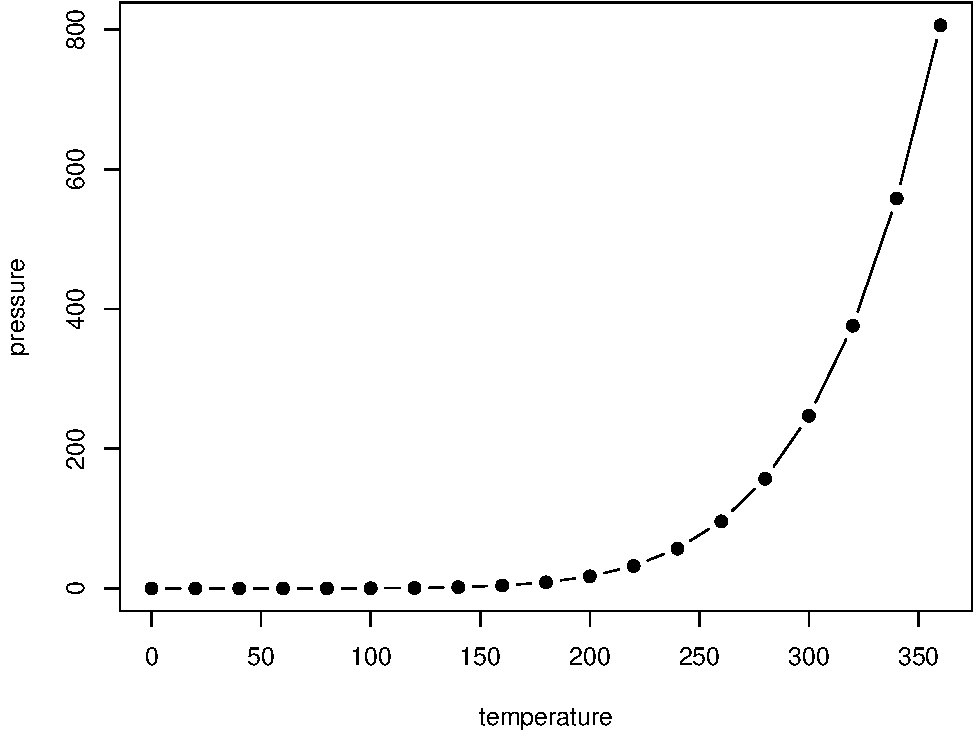
\includegraphics[width=0.8\linewidth]{01-theGolemOfPrague_files/figure-latex/nice-fig-1} 

}

\caption{Here is a nice figure!}\label{fig:nice-fig}
\end{figure}

Reference a figure by its code chunk label with the \texttt{fig:} prefix, e.g., see Figure \ref{fig:nice-fig}. Similarly, you can reference tables generated from \texttt{knitr::kable()}, e.g., see Table \ref{tab:nice-tab}.

\begin{Shaded}
\begin{Highlighting}[]
\NormalTok{knitr}\OperatorTok{::}\KeywordTok{kable}\NormalTok{(}
  \KeywordTok{head}\NormalTok{(iris, }\DecValTok{20}\NormalTok{), }\DataTypeTok{caption =} \StringTok{'Here is a nice table!'}\NormalTok{,}
  \DataTypeTok{booktabs =} \OtherTok{TRUE}
\NormalTok{)}
\end{Highlighting}
\end{Shaded}

\begin{table}

\caption{\label{tab:nice-tab}Here is a nice table!}
\centering
\begin{tabular}[t]{rrrrl}
\toprule
Sepal.Length & Sepal.Width & Petal.Length & Petal.Width & Species\\
\midrule
5.1 & 3.5 & 1.4 & 0.2 & setosa\\
4.9 & 3.0 & 1.4 & 0.2 & setosa\\
4.7 & 3.2 & 1.3 & 0.2 & setosa\\
4.6 & 3.1 & 1.5 & 0.2 & setosa\\
5.0 & 3.6 & 1.4 & 0.2 & setosa\\
\addlinespace
5.4 & 3.9 & 1.7 & 0.4 & setosa\\
4.6 & 3.4 & 1.4 & 0.3 & setosa\\
5.0 & 3.4 & 1.5 & 0.2 & setosa\\
4.4 & 2.9 & 1.4 & 0.2 & setosa\\
4.9 & 3.1 & 1.5 & 0.1 & setosa\\
\addlinespace
5.4 & 3.7 & 1.5 & 0.2 & setosa\\
4.8 & 3.4 & 1.6 & 0.2 & setosa\\
4.8 & 3.0 & 1.4 & 0.1 & setosa\\
4.3 & 3.0 & 1.1 & 0.1 & setosa\\
5.8 & 4.0 & 1.2 & 0.2 & setosa\\
\addlinespace
5.7 & 4.4 & 1.5 & 0.4 & setosa\\
5.4 & 3.9 & 1.3 & 0.4 & setosa\\
5.1 & 3.5 & 1.4 & 0.3 & setosa\\
5.7 & 3.8 & 1.7 & 0.3 & setosa\\
5.1 & 3.8 & 1.5 & 0.3 & setosa\\
\bottomrule
\end{tabular}
\end{table}

You can write citations, too. For example, we are using the \textbf{bookdown} package \citep{R-bookdown} in this sample book, which was built on top of R Markdown and \textbf{knitr} \citep{xie2015}.

  \bibliography{book.bib}

\end{document}
